
\section{Experimentations}

\begin{figure*}
  \centering
  \subfloat[Comportement d'édition attendu]
  [\label{fig:compliant}Le comportement d'édition correspond aux attentes
  de la stratégie d'allocation]
  {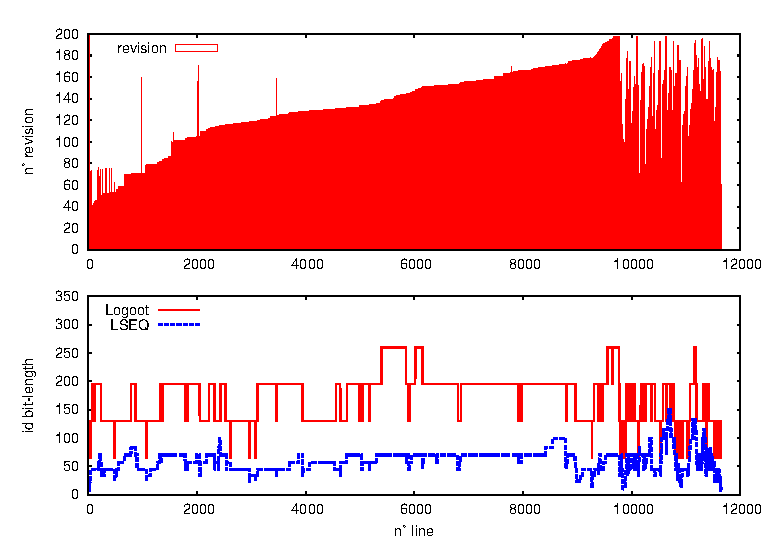
\includegraphics[width=0.48\textwidth]{./img/poste.eps}}
  \hspace{10pt}
  \subfloat[Comportement d'édition inattendu]
  [\label{fig:motivating}Le comportement d'édition va à l'encontre des attentes
  de la stratégie d'allocation]
  {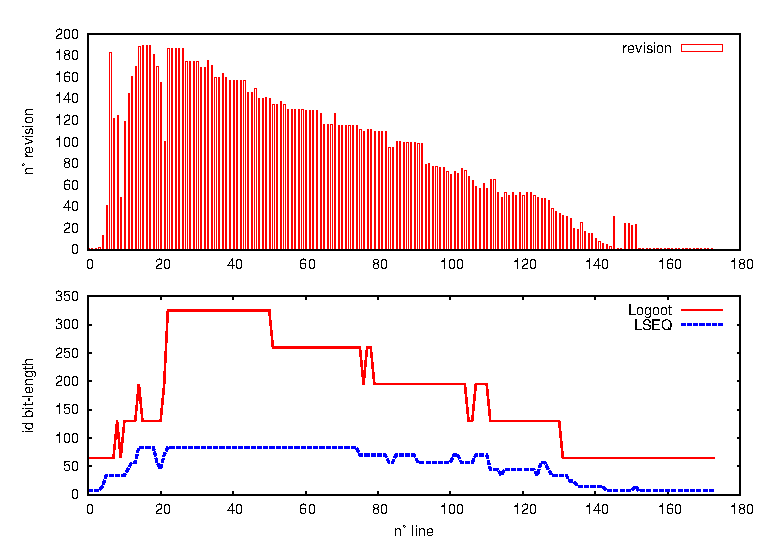
\includegraphics[width=0.48\textwidth]{./img/didyouknow.eps}}
  \caption{\label{fig:allocation}Spectre de document Wikipedia sous différent
    comportements d'édition antagonistes. La figure du haut représente la
    révision à laquelle la ligne a été inséré, i.e., sa date de naissance.  La
    figure du bas représente la taille de l'identifiant associé à chaque ligne.}
\end{figure*}



%%% Local Variables:
%%% mode: latex
%%% TeX-master: "../../paper"
%%% End:
